\section{Experiments}
\subsection{Experimental Setups}
\subsubsection{Datasets}
We conduct experiments on six real-world tabular datasets: Adult~\cite{adult_2}, Anxiety~\cite{kaggleSocialAnxiety}, Compas~\cite{propublicaMachineBias}, Salary~\cite{kaggleGlobalMarket}, Obesity~\cite{obesity}, and Churn~\cite{churn}. These datasets cover a range of domains (e.g., social, medical, business) and downstream tasks including binary/multi-class classification and regression. Notably, Anxiety and Salary were released after the knowledge cutoff of modern LLMs, allowing us to assess performance in the absence of prior exposure. The characteristics of all datasets are summarized in Table~\ref{tab:dataset_summary}. We randomly split each dataset into training and test sets using an 8:2 ratio, yielding $\mathcal{D}_\mathtt{train\text{-}full}$ and $\mathcal{D}_\mathtt{test}$. To simulate data-scarce settings, we further subsample $n$ instances from $\mathcal{D}_\mathtt{train\text{-}full}$ to form the final training set, $\mathcal{D}_\mathtt{train}$. This procedure is repeated ten times with different random seeds (42--51) to ensure robustness.

Additionally, for evaluating structure discovery quality, we utilize three benchmark datasets from bnlearn~\cite{scutari2010learning} with known ground-truth DAGs: Asia~\cite{bnlearn-repo-asia} (8 nodes), Child~\cite{bnlearn-repo-child} (20 nodes), and Insurance~\cite{bnlearn-repo-insurance} (27 nodes). These allow direct measurement of structural recovery via the Structural Hamming Distance (SHD)~\cite{de2009comparison}.

\begin{table*}[ht]
\centering
\caption{Summary of Dataset Characteristics.}
\label{tab:dataset_summary}
\begin{tabular}{lcccccc}
\toprule
\textbf{Dataset} & \textbf{\# Num Feat.} & \textbf{\# Cat Feat.} & \textbf{\# Classes} & \textbf{Domain} & \textbf{Task} & \textbf{Pre-LLM Knowledge Cutoff} \\
\midrule
Adult~\cite{adult_2} & 4 & 11 & 2 & Social/Census & Binary & \textcolor{darksalmon}{\XSolidBrush} \\
Anxiety~\cite{kaggleSocialAnxiety} & 12 & 7 & 3 & Medical/Health & Multi-Class & \textcolor{green(pigment)}{\Checkmark} \\
Compas~\cite{propublicaMachineBias} & 5 & 3 & 2 & Crime & Binary & \textcolor{darksalmon}{\XSolidBrush} \\
Salary~\cite{kaggleGlobalMarket} & 3 & 15 & - & Economy & Regression & \textcolor{green(pigment)}{\Checkmark} \\
Obesity~\cite{obesity} & 7 & 8 & - & Medical/Health & Regression & \textcolor{darksalmon}{\XSolidBrush} \\
Churn~\cite{churn} & 8 & 4 & 2 & Business & Binary & \textcolor{darksalmon}{\XSolidBrush} \\
\bottomrule
\end{tabular}
\end{table*}

\subsubsection{Baselines}
We compare our method against eleven baselines from three categories: 1)~\textbf{Deep Generative Models (DGMs)}, including TVAE~\cite{xu2019modeling}, CTGAN~\cite{xu2019modeling}, TabDDPM~\cite{kotelnikov2023tabddpm}, NFlow~\cite{papamakarios2021normalizing}, and TabSyn~\cite{tabsyn}; 2)~\textbf{Structure-Aware Methods}, including Bayesian Networks~\cite{ankan2015pgmpy}, GOGGLE~\cite{liu2023goggle}, and DECAF~\cite{van2021decaf}; and 3)~\textbf{LLM-based Methods}, including GReaT~\cite{borisov2023language}, CLLM~\cite{cllm2024}, and GraDe~\cite{zhang-etal-2025-features}. For all baseline methods, with the exception of CuratedLLM, we utilize the implementations provided in the SynthCity~\cite{qian2023synthcity} library. These models were run using their default hyperparameter configurations to ensure a standardized comparison. For CuratedLLM, we used the official source code provided by the authors, adapting it to our experimental setup. To ensure a fair comparison, it was configured with the same Large Language Model (LLM) settings as our proposed \textsf{StructSynth}, with detailed parameters provided in Table~\ref{tab:hyperparameters}.

\subsubsection{Evaluation Metrics}
Following previous methods~\cite{borisov2023language, cllm2024}, we evaluate the quality of synthetic data using three metrics:

\paragraph{Downstream Model Performance.}
This metric serves as the primary measure of the synthetic data's practical utility. For each generative method, we create an augmented training set $\mathcal{D}_{\text{aug}} = \mathcal{D}_{\text{train}} \cup \mathcal{D}_{\text{synth}}$. A downstream machine learning model (XGBoost) is trained exclusively on $\mathcal{D}_{\text{aug}}$ and evaluated on the held-out real test set $\mathcal{D}_{\text{test}}$. We report the Area Under the Receiver Operating Characteristic Curve (AUC) for classification tasks and the R-squared ($R^2$) score for regression tasks. Higher scores in either metric signify greater downstream utility.

\paragraph{Statistical Fidelity.}
This metric quantifies how well the synthetic data preserves the pairwise statistical relationships present in the real data. The metric is computed as the mean absolute difference across all pairs of columns, where the specific correlation measure depends on the data types involved: Pearson correlation for numerical-numerical pairs, Total Variation Distance (TVD) of joint distributions for categorical-categorical pairs, and TVD after quantile-based discretization for numerical-categorical pairs. The overall score is:
\begin{equation}
    \text{StatisticalFidelity} = \frac{1}{\binom{K}{2}} \sum_{1 \le i < j \le K} \Delta(C_i, C_j)
\end{equation}
where $K$ is the total number of columns. A \textbf{lower score indicates higher fidelity}.

\paragraph{Privacy Risk Assessment.}
This metric evaluates the extent to which a generative model memorizes the training data. For each synthetic sample $\tilde{x} \in \mathcal{D}_{\text{synth}}$, we identify its nearest neighbor from the complete real data $\mathcal{D}_{\text{real}} = \mathcal{D}_{\text{train}} \cup \mathcal{D}_{\text{test}}$, using a distance function combining L1 distance for numerical features and Hamming distance for categorical features:
\begin{equation}
    d(x_i, x_j) = \sum_{k \in \text{num}} |x_{i,k} - x_{j,k}| + \sum_{l \in \text{cat}} \mathbb{I}(x_{i,l} \neq x_{j,l})
\end{equation}
The Privacy Risk score is the fraction of synthetic samples whose nearest neighbor originates from $\mathcal{D}_{\text{train}}$:
\begin{equation}
    \text{PrivacyRisk} = \frac{1}{|\mathcal{D}_{\text{synth}}|} \sum_{\tilde{x} \in \mathcal{D}_{\text{synth}}} \mathbb{I}(NN(\tilde{x}) \in \mathcal{D}_{\text{train}})
\end{equation}
A \textbf{value approaching 0.5 indicates better privacy preservation}~\cite{van2023membership}, implying that the synthetic data is statistically equidistant to both training and test sets.

\subsubsection{Implementation Details}
\label{sec:implementation}

We use \texttt{gpt-4o-mini} with a temperature of 0.9 for both the CLLM and \textsf{StructSynth} models. Our experiments evaluate the low-data regime, generating 1000 synthetic samples ($s=1000$) from 100 original samples ($n=100$). Downstream performance is assessed using an XGBoost model. All experiments are repeated 10 times, and we report results as mean $\pm$ standard deviation to ensure robustness. For the software implementation, we utilize the Langchain library to manage LLM inference and the Causal-Learn library~\cite{zheng2024causal} for the PC algorithm. The detailed hyperparameter configurations are provided in Table~\ref{tab:hyperparameters}.

\begin{table}[htbp]
\centering
\caption{Hyperparameter Settings for Our Experiments.}
\label{tab:hyperparameters}
\begin{tabular}{ll}
    \toprule
    \textbf{Group} & \textbf{Hyperparameter Settings} \\
    \midrule
    \multirow{5}{*}{LLMs} & frequency\_penalty = 0 \\
    & presence\_penalty = 0 \\
    & top\_p = 0.95 \\
    & temperature = 0.9 \\
    & max\_tokens = 8000 \\
    \midrule
    \multirow{10}{*}{XGBoost} & booster = gbtree \\
    & n\_estimators = 100 \\
    & learning\_rate = 0.1 \\
    & max\_depth = 6 \\
    & min\_child\_weight = 1 \\
    & gamma = 0 \\
    & subsample = 1 \\
    & colsample\_bytree = 1 \\
    & reg\_alpha = 0 \\
    & reg\_lambda = 1 \\
    \midrule
    \multirow{3}{*}{PC algorithm} & alpha = 0.05 \\
    & indep\_test = `kci' \\
    & stable = True \\
    \bottomrule
\end{tabular}
\end{table}


\begin{table*}[ht]
\small
\centering

\setlength{\tabcolsep}{1mm} 
\caption{Comparison of Models on Privacy Preservation and Statistical Fidelity (\%). $^\dag$ indicates datasets created post LLM knowledge cutoff. Best results are in \textbf{bold}; second-best are \underline{underlined}.}

\begin{tabular}{ll|llllll|c|c}
\toprule

\textbf{Type} & \textbf{Method} & 
\multicolumn{1}{c}{\textbf{Adult}} &
\multicolumn{1}{c}{\textbf{Anxiety$^\dag$}} &
\multicolumn{1}{c}{\textbf{Compas}} &
\multicolumn{1}{c}{\textbf{Salary$^\dag$}} &
\multicolumn{1}{c}{\textbf{Obesity}} &
\multicolumn{1}{c}{\textbf{Churn}} &
\textbf{Average} & \textbf{Avg. Rank} \\

\midrule
\multicolumn{10}{l}{{Results for \textbf{Privacy Preservation}.} \textit{A value approaching 0.5 indicates better privacy preservation.}} \\
\midrule
    \multirow{5}{*}{DGMs} & TVAE & \underline{$50.34_{\pm 3.91}$} & $55.41_{\pm 4.26}$ & $64.50_{\pm 5.18}$ & $55.09_{\pm 4.38}$ & $52.93_{\pm 7.86}$ & $58.70_{\pm 4.75}$ & $56.16$ & $4.33$ \\
    & DDPM & $99.95_{\pm 0.05}$ & $66.20_{\pm 13.17}$ & $67.18_{\pm 18.06}$ & $63.32_{\pm 19.52}$ & $71.36_{\pm 16.88}$ & $62.89_{\pm 24.91}$ & $71.82$ & $9.67$ \\
    & CTGAN & $50.70_{\pm 3.64}$ & $56.64_{\pm 4.72}$ & $64.43_{\pm 4.22}$ & $53.59_{\pm 2.05}$ & $53.44_{\pm 3.89}$ & $57.84_{\pm 2.31}$ & $56.11$ & $4.67$ \\
    & NFlow & $54.36_{\pm 1.92}$ & $\boldsymbol{53.52_{\pm 3.08}}$ & \underline{$62.57_{\pm 3.66}$} & $52.76_{\pm 2.34}$ & $51.74_{\pm 3.68}$ & $52.97_{\pm 3.33}$ & $54.65$ & $3.50$ \\
    & TabSyn & $51.64_{\pm 2.67}$ & $70.53_{\pm 7.45}$ & $67.55_{\pm 5.40}$ & $54.66_{\pm 4.19}$ & $63.30_{\pm 7.19}$ & $59.38_{\pm 3.70}$ & $61.18$ & $7.50$ \\
\midrule
    \multirow{3}{*}{\makecell[l]{Structure\\Aware}} & GOGGLE & $49.15_{\pm 7.97}$ & $43.62_{\pm 33.49}$ & $65.16_{\pm 17.25}$ & $30.94_{\pm 18.49}$ & $44.28_{\pm 23.83}$ & $61.87_{\pm 18.01}$ & \underline{$49.17$} & $7.17$ \\
    & BN & $53.73_{\pm 2.36}$ & $72.98_{\pm 4.69}$ & $67.78_{\pm 3.63}$ & $61.50_{\pm 1.48}$ & $68.02_{\pm 2.18}$ & $59.68_{\pm 3.74}$ & $63.95$ & $8.83$ \\
    & DECAF & $46.23_{\pm 19.13}$ & $58.59_{\pm 10.37}$ & $64.07_{\pm 19.14}$ & $56.91_{\pm 17.41}$ & \underline{$50.82_{\pm 15.49}$} & $69.79_{\pm 18.81}$ & $57.74$ & $6.33$ \\
    \midrule
    \multirow{3}{*}{LLMs} & GReaT & $99.50_{\pm 0.35}$ & $85.39_{\pm 2.29}$ & $94.10_{\pm 1.33}$ & $86.66_{\pm 2.45}$ & $80.75_{\pm 2.99}$ & $94.51_{\pm 1.48}$ & $90.15$ & $11.83$ \\
    & CLLM & $49.45_{\pm 3.85}$ & $44.37_{\pm 4.55}$ & $64.14_{\pm 4.22}$ & \underline{$50.96_{\pm 5.40}$} & $45.36_{\pm 2.69}$ & $\boldsymbol{48.78_{\pm 5.82}}$ & $\boldsymbol{50.51}$ & \underline{$3.33$} \\
    & GraDe & $97.51_{\pm 1.60}$ & $61.14_{\pm 1.94}$ & $75.11_{\pm 5.11}$ & $65.99_{\pm 2.60}$ & $59.30_{\pm 4.76}$ & $69.07_{\pm 2.86}$ & $71.35$ & $9.50$ \\
    \midrule
    \multirow{1}{*}{Ours} & StructSynth & $\boldsymbol{49.97_{\pm 5.78}}$ & \underline{$44.74_{\pm 5.13}$} & $\boldsymbol{62.37_{\pm 3.86}}$ & $\boldsymbol{50.13_{\pm 4.89}}$ & $\boldsymbol{49.80_{\pm 6.31}}$ & \underline{$48.67_{\pm 4.84}$} & $50.95$ & $\boldsymbol{1.33}$ \\

\bottomrule
\toprule
\multicolumn{10}{l}{{Results for \textbf{Statistical Fidelity}.} \textit{A lower score indicates higher fidelity.}} \\
\midrule
    \multirow{5}{*}{DGMs} & TVAE & $53.71_{\pm 1.80}$ & $46.16_{\pm 1.28}$ & $60.26_{\pm 1.09}$ & $66.93_{\pm 1.13}$ & \underline{$58.41_{\pm 0.52}$} & $53.22_{\pm 1.54}$ & $58.11$ & $5.17$ \\
    & DDPM & $65.26_{\pm 1.05}$ & $52.76_{\pm 1.22}$ & $64.94_{\pm 1.79}$ & $90.51_{\pm 0.33}$ & $64.44_{\pm 1.36}$ & $64.40_{\pm 2.90}$ & $67.05$ & $10.00$ \\
    & CTGAN & \underline{$52.37_{\pm 1.56}$} & $47.14_{\pm 2.39}$ & $59.96_{\pm 0.90}$ & $58.57_{\pm 0.89}$ & $58.71_{\pm 0.57}$ & \underline{$52.32_{\pm 1.75}$} & $54.85$ & \underline{$4.17$} \\
    & NFlow & $\boldsymbol{50.68_{\pm 2.71}}$ & \underline{$43.50_{\pm 1.77}$} & $60.62_{\pm 0.93}$ & \underline{$52.38_{\pm 1.10}$} & $58.85_{\pm 0.98}$ & $53.98_{\pm 2.24}$ & $\boldsymbol{53.34}$ & $4.50$ \\
    & TabSyn & $49.17_{\pm 1.34}$ & $55.31_{\pm 1.31}$ & $57.23_{\pm 2.24}$ & $62.90_{\pm 3.01}$ & $58.08_{\pm 0.54}$ & $53.99_{\pm 2.08}$ & $56.11$ & $4.75$ \\
\midrule
    \multirow{3}{*}{\makecell[l]{Structure\\Aware}} & GOGGLE & $68.32_{\pm 1.38}$ & $51.58_{\pm 7.27}$ & $66.19_{\pm 1.13}$ & $87.15_{\pm 1.65}$ & $63.80_{\pm 2.40}$ & $65.51_{\pm 2.16}$ & $67.09$ & $10.00$ \\
    & BN & $82.68_{\pm 1.35}$ & $82.77_{\pm 2.39}$ & $60.13_{\pm 3.46}$ & $\boldsymbol{46.33_{\pm 7.29}}$ & $59.76_{\pm 3.46}$ & $88.85_{\pm 3.02}$ & $70.09$ & $8.17$ \\
    & DECAF & $62.71_{\pm 3.21}$ & $48.53_{\pm 1.53}$ & $63.82_{\pm 1.34}$ & $84.70_{\pm 2.41}$ & $60.93_{\pm 2.21}$ & $60.22_{\pm 0.88}$ & $63.49$ & $8.17$ \\
    \midrule
    \multirow{3}{*}{LLMs} & GReaT & $82.71_{\pm 1.35}$ & $\boldsymbol{40.10_{\pm 1.64}}$ & $\boldsymbol{52.17_{\pm 1.18}}$ & $58.75_{\pm 0.89}$ & $\boldsymbol{56.83_{\pm 0.87}}$ & $\boldsymbol{48.18_{\pm 2.16}}$ & \underline{$56.46$} & $\boldsymbol{3.33}$ \\
    & CLLM & $61.93_{\pm 4.43}$ & $57.64_{\pm 1.51}$ & $59.74_{\pm 2.33}$ & $78.60_{\pm 0.98}$ & $65.74_{\pm 1.42}$ & $62.20_{\pm 3.68}$ & $64.31$ & $8.50$ \\
    & GraDe & $84.30_{\pm 0.86}$ & $42.59_{\pm 0.93}$ & $53.82_{\pm 2.62}$ & $55.85_{\pm 1.42}$ & $57.44_{\pm 1.43}$ & $53.66_{\pm 1.90}$ & $57.94$ & \underline{$4.17$} \\
    \midrule
    Ours & StructSynth & $57.60_{\pm 3.13}$ & $57.86_{\pm 1.98}$ & \underline{$57.23_{\pm 1.69}$} & $64.64_{\pm 0.96}$ & $61.14_{\pm 1.10}$ & $58.63_{\pm 2.66}$ & $59.52$ & $7.08$ \\
\bottomrule
\end{tabular}
\label{tab:results_comparison_merged}

\end{table*}

\subsection{Main Results}
\subsubsection{Downstream Model Performance}
We evaluate the generated data on downstream tasks and, for comparison, also report results using the original limited training set $\mathcal{D}_\mathtt{train}$. The results are summarized in Table~\ref{tab:results_comparison_performance}. Our method, \textsf{StructSynth}, consistently outperforms all baselines across all datasets, achieving a perfect average rank of 1.00 and the highest average score (75.01). This provides a significant improvement over using only the original $\mathcal{D}_\mathtt{train}$ (71.54) and surpasses the strongest competitor, CLLM (73.36), demonstrating that explicitly guiding an LLM with a structural blueprint yields substantial gains. Concurrently, the weaker performance of standard DGMs (e.g., TabSyn) and prior structure-aware models (e.g., GOGGLE) validates our core hypotheses: implicit learning is unreliable with sparse data, and generative performance is crippled if the initial structure discovery fails. These findings strongly confirm that \textsf{StructSynth}'s decoupled design, which unifies robust structure learning with LLM-based generation, is a more effective approach for high-fidelity data synthesis in low-data regimes.



\subsubsection{Privacy Preservation and Statistical Fidelity}

We evaluate each generative model on the competing objectives of statistical fidelity and privacy preservation to analyze this critical trade-off (Table~\ref{tab:results_comparison_merged}).

\paragraph{Privacy Preservation.}
\textsf{StructSynth} achieves the best privacy preservation among all models (avg.\ rank 1.33), closely matched only by CLLM (avg.\ rank 3.33). This strong privacy performance is attributable to our decoupled framework: by conditioning generation on the discovered structural blueprint rather than directly modeling the training distribution, the framework avoids the record-level overfitting observed in fine-tuning-based methods. In contrast, GReaT exhibits severe memorization with a Privacy Risk of 90.15\%---nearly double the ideal value of 50\%---indicating that its high-fidelity outputs are largely reproductions of training records rather than genuinely novel samples.

\paragraph{Statistical Fidelity: An Instructive Discrepancy.}
A notable and potentially counterintuitive finding is that \textsf{StructSynth} does not achieve the top Statistical Fidelity ranking (avg.\ rank 7.08), despite its explicit modeling of feature dependencies. One might expect that dependency-aware generation would naturally produce better pairwise correlation matching. We argue that this discrepancy is both \emph{expected} and \emph{informative}, and its proper interpretation is essential for understanding the method's design philosophy.

The key insight lies in what Statistical Fidelity actually measures versus what \textsf{StructSynth} optimizes. The fidelity metric quantifies the preservation of \emph{marginal pairwise} correlations across all $\binom{K}{2}$ feature pairs. In contrast, \textsf{StructSynth}'s DAG encodes \emph{conditional} dependencies---the directed probabilistic relationships between parent and child nodes that govern the data-generating process. These two notions of ``faithfulness'' are fundamentally different: preserving conditional dependencies (which drives downstream utility) does not require---and may even conflict with---perfectly replicating marginal pairwise statistics.

This interpretation is supported by two complementary pieces of evidence. First, GReaT, which achieves the best fidelity (avg.\ rank 3.33), does so at the cost of catastrophic privacy violation (90.15\%), revealing that its high pairwise correlation matching is an artifact of memorization rather than genuine distributional learning. Second, our ablation study provides an even more striking illustration: the \textit{Bayesian Sampler} variant achieves the best raw fidelity score in the ablation (48.86) yet produces the \emph{lowest} downstream utility (AUC = 81.17). This conclusively demonstrates that \textbf{high pairwise fidelity does not guarantee---and can even be inversely related to---downstream performance}. These two cases, examined together, show that fidelity scores can be misleading indicators of a generative model's true quality.

In essence, \textsf{StructSynth}'s structural blueprint acts as a \emph{principled regularizer}: it constrains the generation space to follow discovered conditional dependencies, simultaneously preventing memorization (ensuring privacy, avg.\ rank 1.33) and preserving the dependency structure that matters most for downstream tasks (ensuring utility, avg.\ rank 1.00), at the cost of slightly lower marginal pairwise correlation matching. We provide a detailed theoretical analysis of this fidelity-privacy-utility trade-off in Section~\ref{sec:fidelity_discussion}.


\begin{figure*}[t!]
\centering
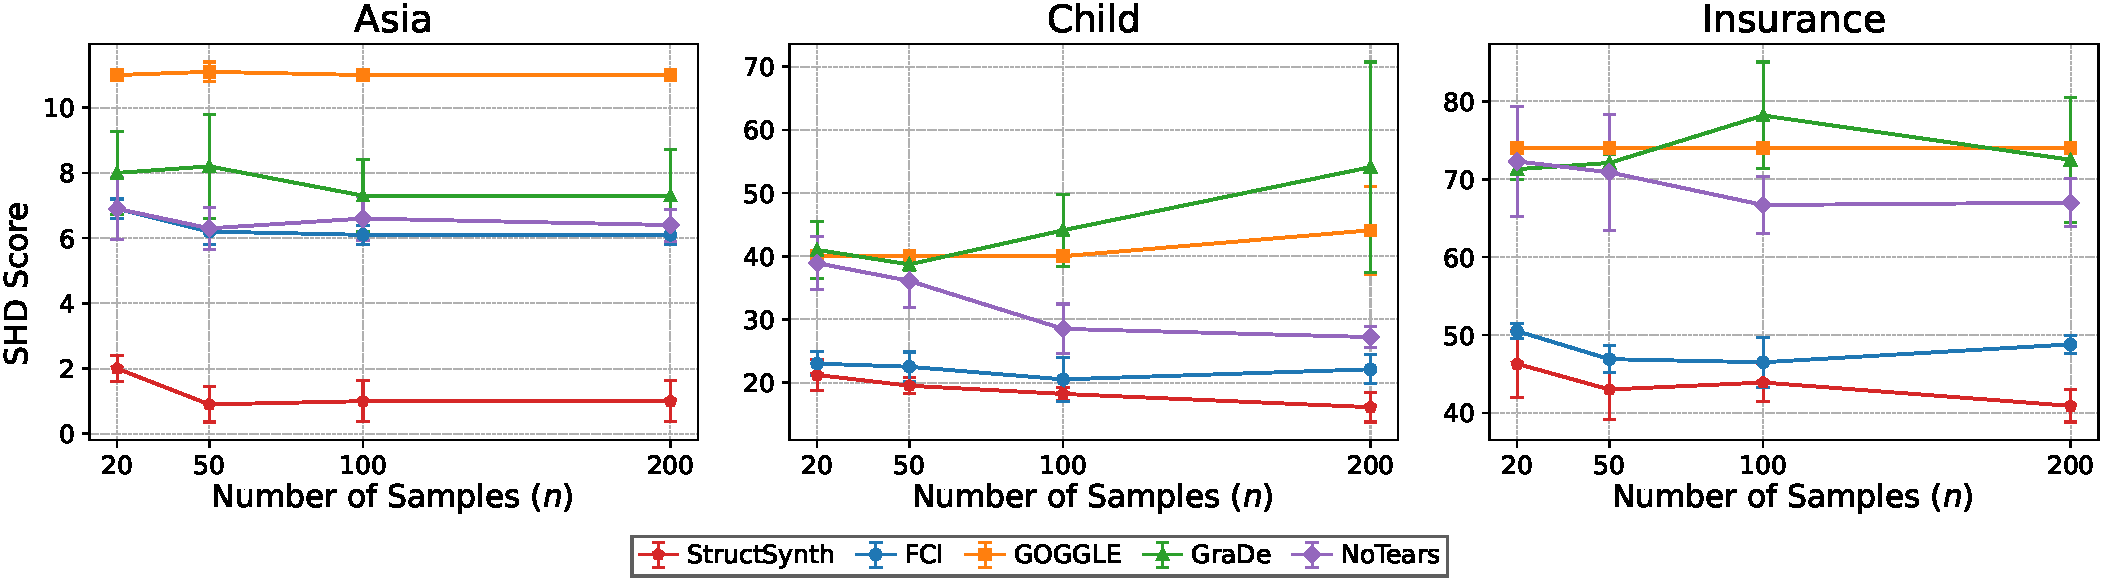
\includegraphics[width=2\columnwidth]{figures/shd_comparison_acm.pdf}
\caption{SHD of discovered dependency graphs vs. number of training samples on Asia, Child, and Insurance datasets with ground-truth DAGs. Lower SHD indicates better structural recovery.}
\label{fig:shd}
\end{figure*}




\subsection{Ablation Study}

To isolate the contributions of our method's two main stages, we evaluate seven variants. For the structure learning stage: 1) \textit{PC Discovery}, substituting our LLM-guided discovery with the classical Peter--Clark algorithm~\cite{spirtes2000causation}; 2) \textit{NoTears Discovery}, replacing our method with the continuous optimization-based NoTears algorithm~\cite{zheng2018dags}; 3) \textit{No-Correlation Score}, removing statistical correlation scores from the prompt to examine their guiding influence; and 4) \textit{Pairwise Discovery}, replacing the efficient BFS traversal with less scalable pairwise queries to evaluate the performance-efficiency trade-off. For the data generation stage: 5) \textit{No Topological Order}, conducting data generation based on the complete learned structure but ignoring the topological order; 6) \textit{No Structure}, removing structural guidance entirely (equivalent to the CLLM); and 7) \textit{Bayesian Sampler}, substituting the LLM generator with a traditional Bayesian sampler fitted to the learned graph.



\begin{table}[t!]
\small
\centering

\caption{Ablation Study on Adult Datasets.}
\setlength{\tabcolsep}{1mm}
\begin{tabular}{ll|ccc}
    \hline
    \multicolumn{2}{c|}{\textbf{Method}} & \textbf{AUC} & \textbf{Fidelity} & \textbf{Privacy} \\ 
    \hline
    \multicolumn{2}{c|}{\textsf{StructSynth}}& \textbf{85.55} & 57.96 & \underline{49.97} \\
    \hline
    \multirow{4}{*}{\makecell[l]{Structure\\Learning}} & PC Discovery& 84.54 & 59.69 & 50.52 \\
    & NoTears Discovery& 84.17 & 59.49 & 47.85 \\
    & No-Correlation Score& 84.06 & 59.10 & 46.60 \\
    & Pairwise Discovery & \underline{85.25} & 57.37 & 49.17 \\
    \hline
    \multirow{3}{*}{Generation} & No Topological Order & 84.41 & 60.47 & 51.03 \\
    & No Structure & 83.95 & 60.67 & 49.45 \\
    & Bayesian Sampler & 81.17 & \textbf{48.86} & \textbf{50.02} \\
    \hline
\end{tabular}

\label{tab:ablation_study}

\end{table}

The results, summarized in Table \ref{tab:ablation_study}, offer three key insights. First, \textbf{LLM-guided discovery outperforms classical structure learning}: \textsf{StructSynth} surpasses both \textit{PC} and \textit{NoTears} (by 1.0--1.4 AUC pts), suggesting that leveraging semantic priors helps identify robust structures in low-data regimes where purely statistical methods suffer from sample instability. Second, \textbf{structural guidance produces a qualitative, not merely quantitative, improvement}: the \textit{No Structure} variant is \emph{operationally equivalent to CLLM}---it uses exactly the same LLM with identical hyperparameters, differing \emph{only} in the absence of structural guidance. The 1.6-point AUC gap between StructSynth and this variant therefore isolates the precise contribution of the discovered dependency graph: it represents how much performance is gained purely from knowing and enforcing feature dependencies. Removing the topological ordering alone (\textit{No Topological Order}) accounts for 1.1 of these 1.6 points, demonstrating that the correct conditioning order---not just the existence of a graph---is critical for generation quality. Third, \textbf{synergy between structure and LLM is irreplaceable}: replacing the LLM generator with a \textit{Bayesian Sampler} fitted to the same learned graph causes the sharpest drop (--4.4 pts AUC to 81.17), despite the sampler achieving the best raw fidelity score (48.86). This result is doubly informative: it confirms that the structural blueprint effectively guides---but cannot replace---the LLM's superior distributional learning, and it demonstrates that high pairwise fidelity alone does not guarantee downstream utility ($\text{Fidelity}=48.86$ yet $\text{AUC}=81.17$, the lowest among all variants). Additionally, removing statistical prompts (\textit{No-Correlation}) degrades performance by 1.5 pts, highlighting their value as weak supervision that anchors the LLM's semantic reasoning in empirical evidence. Taken together, these ablations demonstrate that each component of \textsf{StructSynth}---LLM-guided discovery, topological generation ordering, and statistical grounding---makes a non-trivial, independently measurable contribution. The consistent degradation from removing any single component (ranging from 1.0 to 4.4 AUC points) confirms that these are \emph{structural design choices} that fundamentally change how the generation process operates, rather than superficial additions to an existing pipeline. A detailed discussion on how these components collectively distinguish StructSynth from structure-blind LLM methods is provided in Section~\ref{sec:structure_discussion}.


% The results, summarized in Table \ref{tab:ablation_study}, confirm that the framework's success stems from the synergy between the discovered graph and the LLM's generative power. Our central finding is that graph awareness is critical. Removing the structural guidance (\textit{No Structure}) significantly reduces AUC by 1.6 pts. More dramatically, replacing the LLM with a Bayesian Sampler yields the largest performance drop (–4.4 pts). This confirms the vital synergy between the learned graph and the LLM's generative capabilities—neither component is sufficient in isolation. We also find that prompt signals matter, as using \textit{No-Correlation} degrades AUC by 1.5 pts, highlighting their utility as a form of weak supervision.



\subsection{Structural Fidelity under Ground-Truth Graphs}

To rigorously evaluate the quality of the discovered structures, we employ three benchmark datasets from the \texttt{bnlearn} repository---Asia, Child, and Insurance---which possess known ground-truth DAGs. This allows us to directly quantify structural fidelity using the Structural Hamming Distance (SHD), which is standard in the literature and measures the number of edge insertions, deletions, or reversals required to transform the learned graph into the ground truth. A lower SHD indicates a more accurate recovery of the underlying causal mechanisms.

Figure \ref{fig:shd} presents the SHD across varying training sample sizes ($n \in \{20, 50, 100, 200\}$). \textsf{StructSynth} consistently achieves the lowest or near-lowest SHD across all datasets, demonstrating superior stability in low-data regimes. In contrast, traditional constraint-based methods like FCI and score-based methods like GOGGLE often yield significantly higher errors, particularly when $n$ is small.

On the \textbf{Asia} dataset, which is small but prone to spurious correlations in low-sample settings, \textsf{StructSynth} maintains an SHD near 1, whereas baselines fluctuate at much higher error rates. This suggests that our LLM-guided approach effectively utilizes prior knowledge to filter out false positives that purely statistical methods might mistake for true edges. For the \textbf{Child} dataset, which features a more complex structure, errors in early discovery stages can cascade. \textsf{StructSynth}'s iterative cycle resolution helps maintain graph validity, preventing the explosion of erroneous edges seen in methods like GraDe. Finally, on the \textbf{Insurance} dataset, which represents a medium-scale network with denser connections, our method again outperforms competitors. By prioritizing the discovery of a stable ``structural blueprint'' rather than attempting to model every minor correlation, \textsf{StructSynth} avoids the overfitting pitfalls that lead to the dense, incorrect graphs produced by some deep generative baselines. These results validate the first stage of our framework: \textsf{StructSynth} reliably identifies a high-fidelity dependency structure even from limited data, which is crucial for ensuring the subsequent generation follows valid causal pathways.


\subsection{Qualitative Analysis of Discovered Structures}
\label{sec:qualitative}

\subsubsection{Structural Fidelity on Adult Dataset}

To provide a qualitative illustration of our method's ability to preserve the core dependencies within the data in the absence of a ground-truth graph, we present a case study on the Adult dataset in Figure~\ref{fig:structure}. This visualization compares three distinct graphs: (a) a reference graph, established by running the PC algorithm on the complete dataset and refining the output with domain expertise; (b) the dependency graph discovered by \textsf{StructSynth}'s learning stage from $\mathcal{D}_\mathtt{train}$; and (c) a graph re-discovered from $\mathcal{D}_\mathtt{synth}$ generated by \textsf{StructSynth} using the PC algorithm.

A visual comparison reveals a strong alignment between our LLM-discovered graph (Figure~\ref{fig:structure_llmcd}) and the reference graph (Figure~\ref{fig:structure_groundtruth}), particularly around the key \textit{Salary} variable. This demonstrates the effectiveness of our structure learning phase in creating a high-quality dependency graph. More importantly, the remarkable structural similarity between the re-discovered graph (Figure~\ref{fig:structure_structsynth}) and the reference graph serves as powerful evidence of our method's fidelity. The ability of a standard discovery algorithm to independently recover the essential generative pathways from our synthetic data confirms that \textsf{StructSynth} effectively preserves the underlying dependency structure.

\begin{figure*}[h!]
    \centering
    \begin{subfigure}[b]{0.37\textwidth}
        \centering
        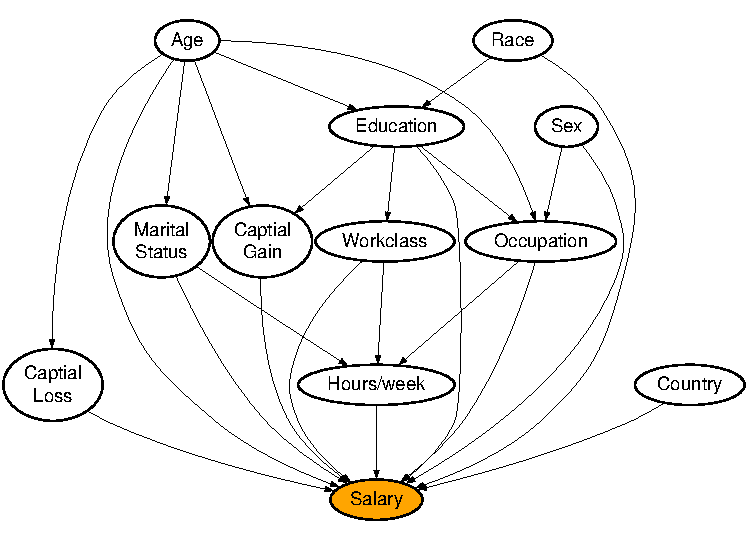
\includegraphics[width=\linewidth]{figures/graph/reference.pdf}
        \caption{Reference Graph}
        \label{fig:structure_groundtruth}
    \end{subfigure}%
    \hfill 
    \begin{subfigure}[b]{0.3\textwidth}
        \centering
        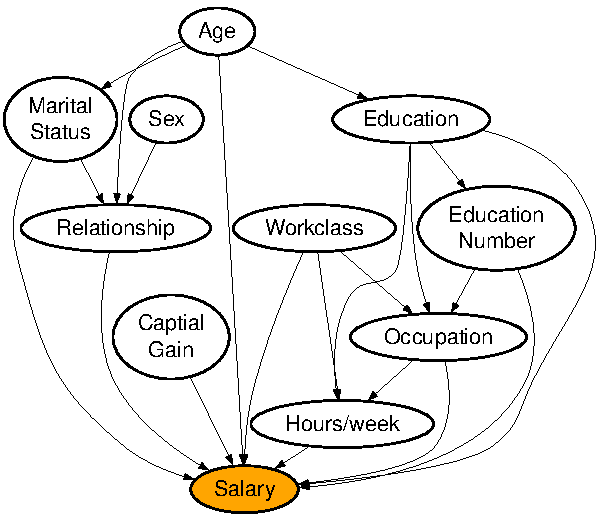
\includegraphics[width=\linewidth]{figures/graph/llm.pdf}
        \caption{LLM-Discovered}
        \label{fig:structure_llmcd}
    \end{subfigure}%
    \hfill 
    \begin{subfigure}[b]{0.32\textwidth}
        \centering
        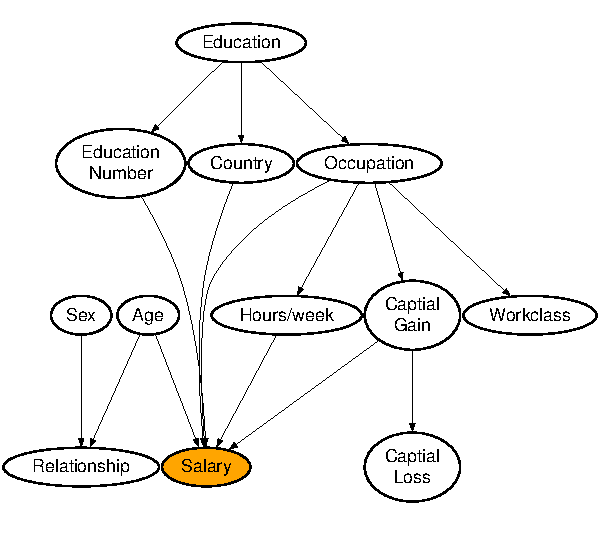
\includegraphics[width=\linewidth]{figures/graph/structsynth.pdf}
        \caption{Re-discovered from Synthetic Data}
        \label{fig:structure_structsynth}
    \end{subfigure}
    \caption{Visual Analysis of Structural Fidelity on the Adult Dataset with \textit{Salary} as the Label Column.}
    \label{fig:structure}
\end{figure*}

\subsubsection{Structure Discovery Comparisons on Asia Dataset}

To provide a concrete illustration of the structural discovery capabilities discussed above, Figure~\ref{fig:structure_examples} presents a visual comparison of the dependency graphs learned by \textsf{StructSynth} and four representative baselines on the Asia dataset ($n=100$). The \textbf{Ground Truth} graph represents the underlying causal mechanism of the dataset, where, for example, \textit{smoke} causes \textit{lung} (cancer) and \textit{bronc} (bronchitis), which in turn cause \textit{dysp} (dyspnoea).

\textsf{StructSynth} successfully recovers the majority of these key dependencies, including the V-structure at \textit{dysp} and the causal chain from \textit{smoke} to \textit{lung}. The slight deviations are minimal and do not disrupt the global topological ordering, ensuring that the subsequent generation process follows a valid causal path.

In contrast, baseline methods exhibit significant structural distortions:
\begin{itemize}[leftmargin=*]
    \item \textbf{GraDe} tends to produce an overly dense graph with numerous spurious edges (e.g., direct links between \textit{asia} and \textit{dysp}), likely due to its reliance on attention maps that can conflate indirect correlations with direct causation.
    \item \textbf{GOGGLE}, while capturing some dependencies, suffers from edge reversals (e.g., \textit{lung} $\rightarrow$ \textit{smoke}) and misses critical connections (e.g., \textit{bronc} is isolated from \textit{dysp}). This reflects the instability of end-to-end differentiable structure learning in low-data regimes.
    \item \textbf{NoTears} yields a sparse and fragmented graph, failing to identify the relationship between \textit{smoke} and \textit{lung}, which are central to the dataset's causal logic.
    \item \textbf{FCI}, a constraint-based method, correctly identifies some skeletons but leaves many edges undirected (represented by bi-directed or unoriented edges), failing to provide a clear generative order.
\end{itemize}

These visual examples corroborate our quantitative findings in Figure~\ref{fig:shd}, confirming that \textsf{StructSynth}'s LLM-guided approach offers superior robustness in discovering interpretable and accurate dependency structures compared to both traditional and deep learning-based alternatives.

\begin{figure*}[t!]
\centering
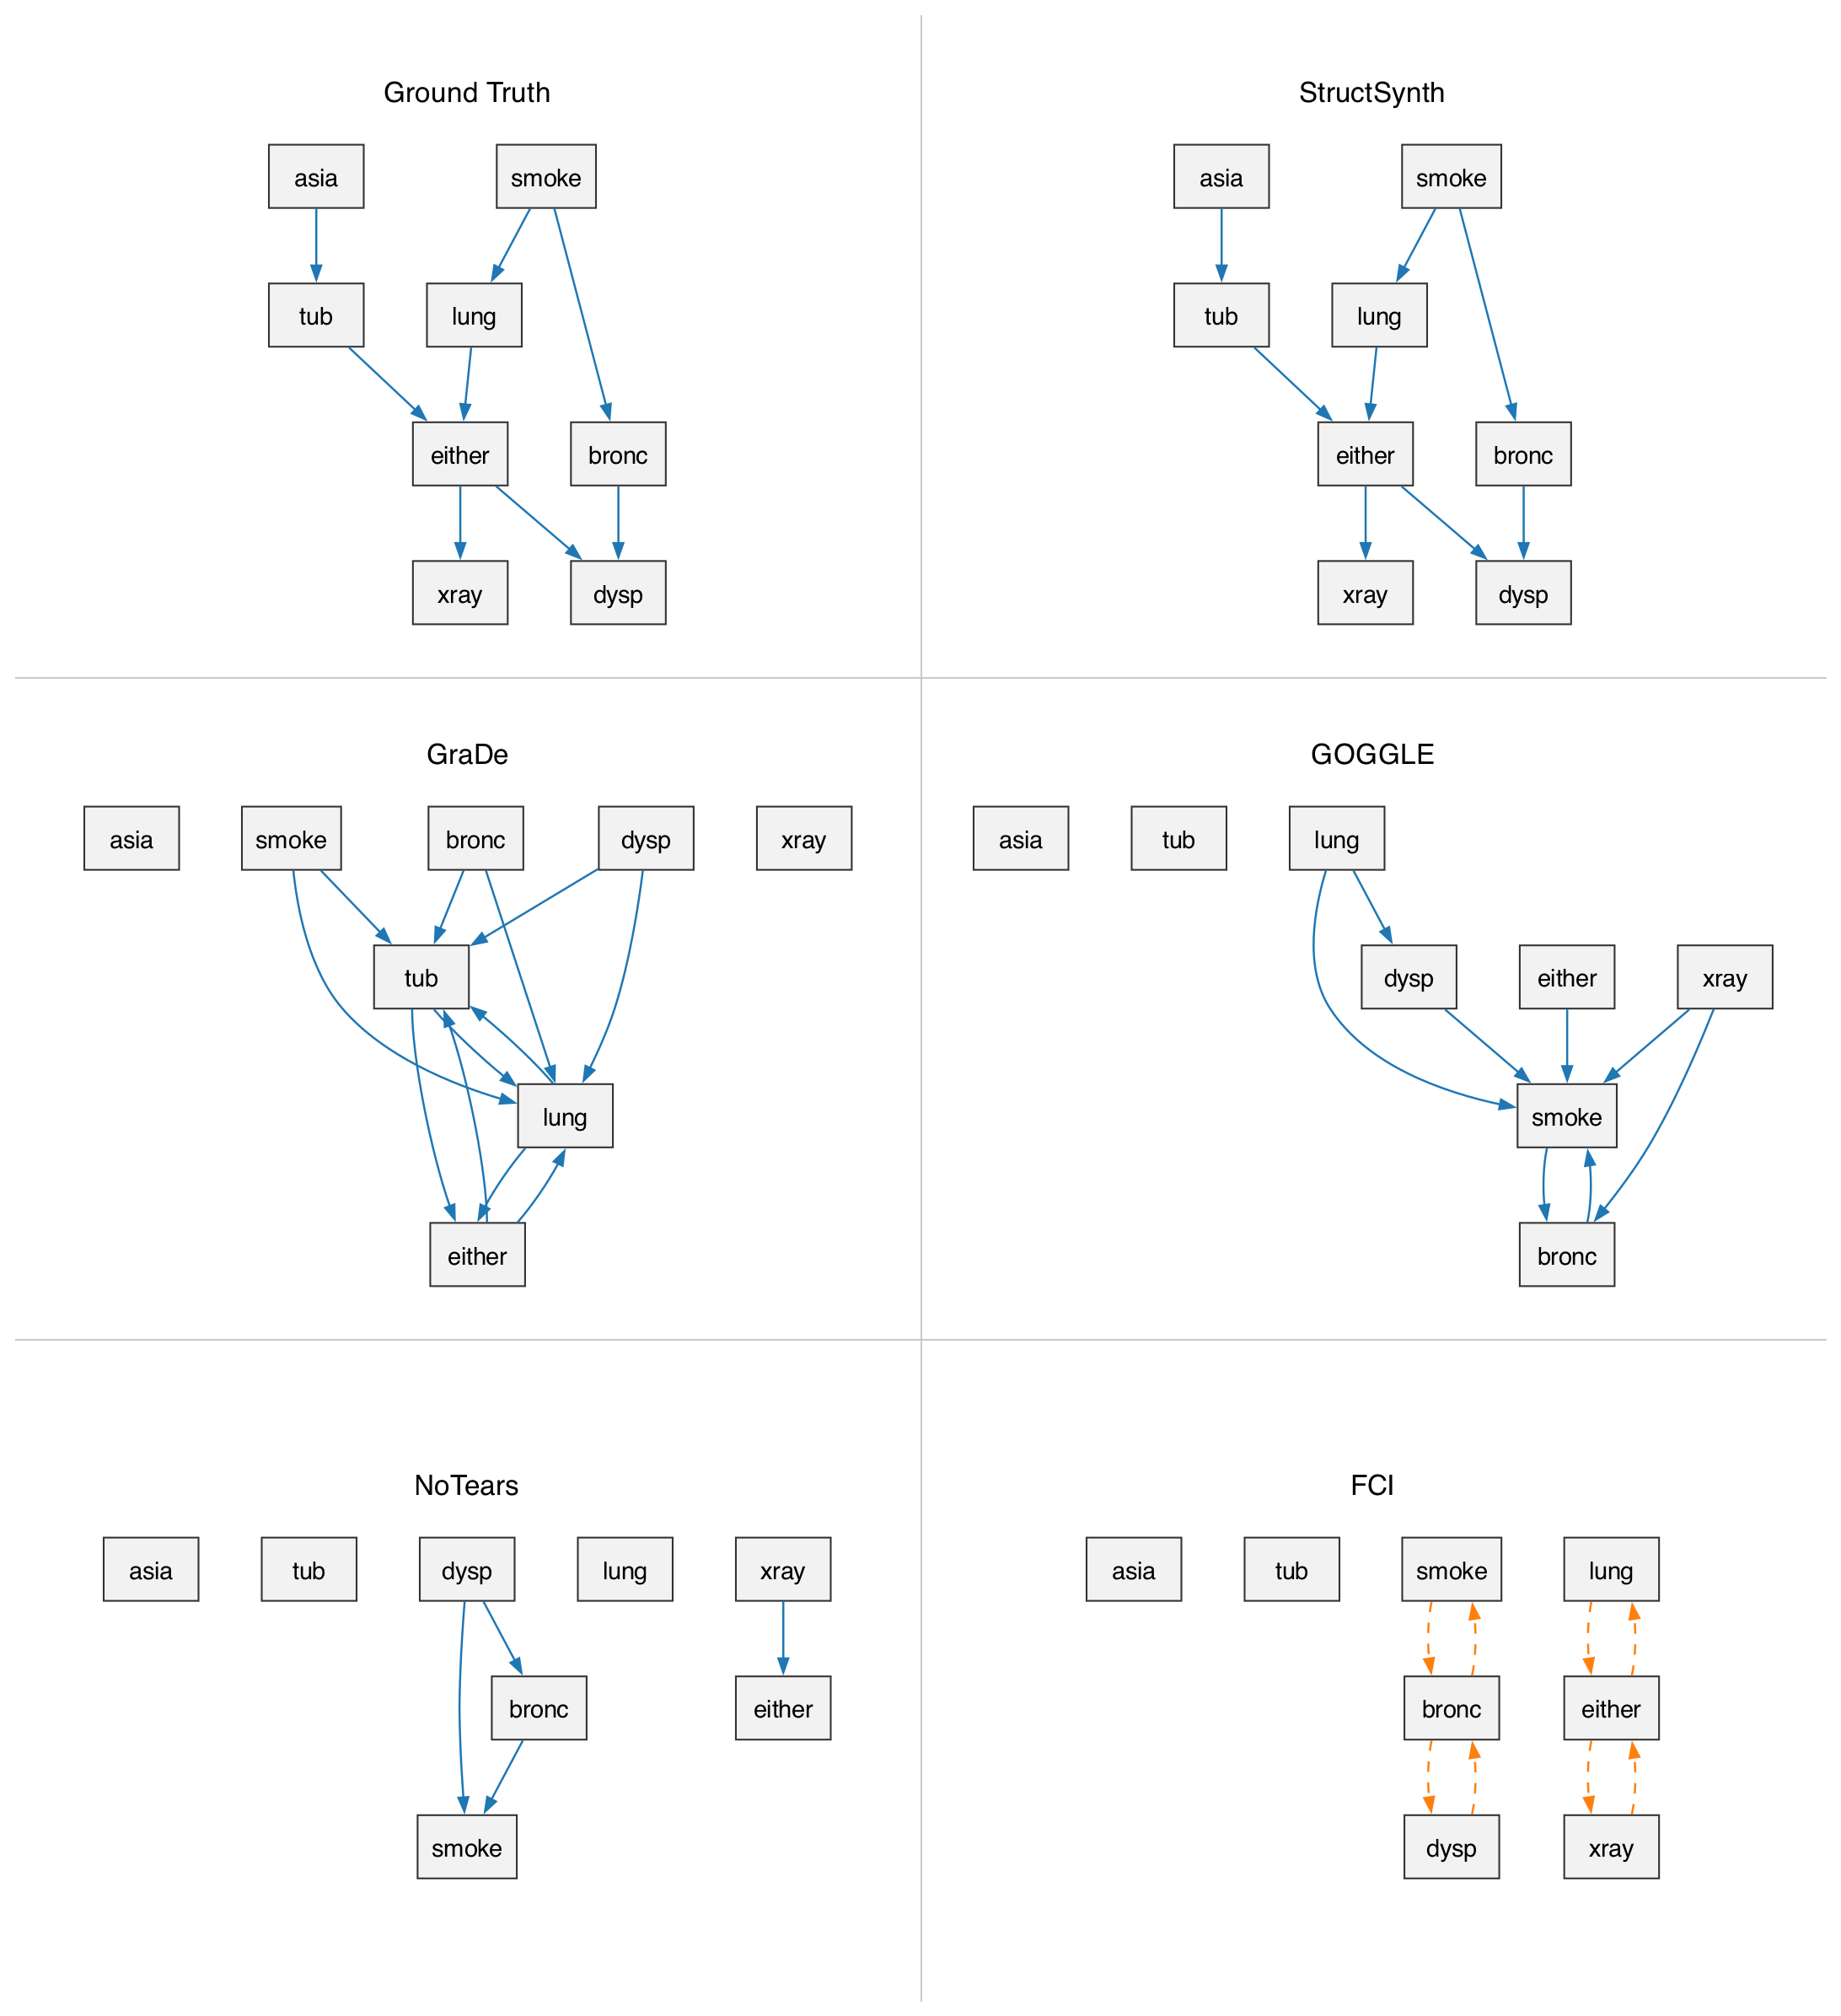
\includegraphics[width=1.8\columnwidth]{figures/collage_3x2.png}
\caption{Comparison of discovered dependency structures on the Asia dataset ($n=100$). \textbf{Ground Truth}: The reference DAG from the bnlearn repository. \textbf{StructSynth}: Our method closely recovers the ground truth. \textbf{GraDe, GOGGLE, NoTears, FCI}: Baseline methods exhibit varying degrees of structural errors, including missing edges, reversed edges, and spurious connections.}
\label{fig:structure_examples}
\end{figure*}


\subsection{Influence of Training Sample Size}

\begin{figure*}[t!]
\centering
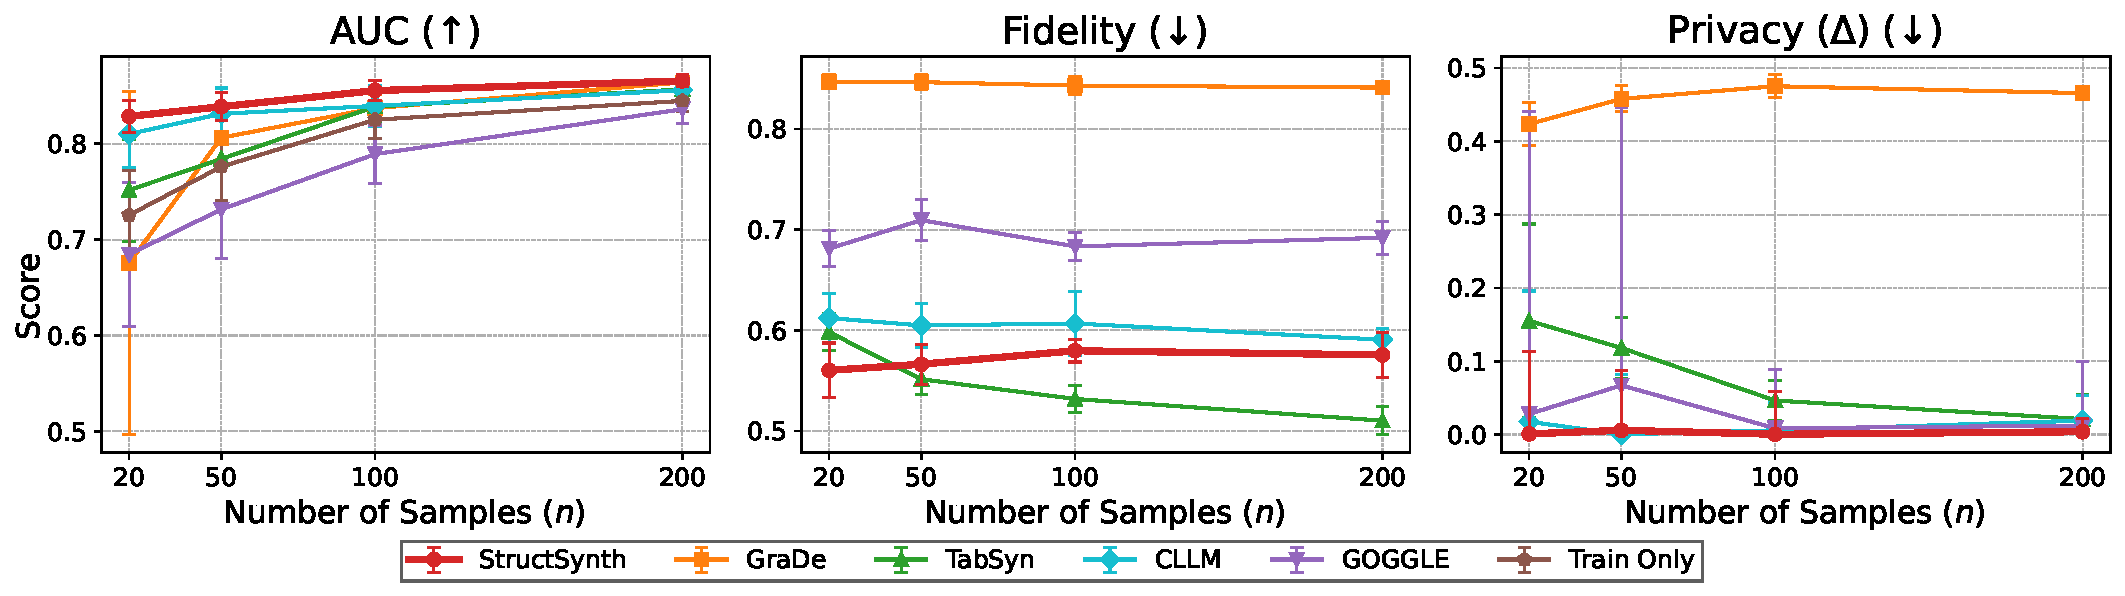
\includegraphics[width=2\columnwidth]{figures/influence_n/vary_n_all.pdf}
\caption{Effect of training sample size ($n$) on downstream utility (AUC$\uparrow$), statistical fidelity ($\downarrow$), and privacy risk deviation $\Delta$ ($\downarrow$) on the Adult dataset.}
\label{fig:influence_n}
\end{figure*}

\begin{figure}[h]
\centering
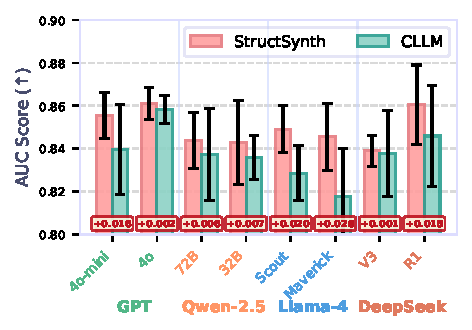
\includegraphics[width=\columnwidth]{figures/llm_compare.pdf}
\caption{AUC Score on the Adult Dataset Using Various LLMs for \textsf{StructSynth} and CLLM.}
\label{fig:llm_compare}
\end{figure}


To evaluate data efficiency, we varied the training size $n$ from 20 to 200 on the Adult dataset and measured AUC, Statistical Fidelity, and Privacy Risk deviation $\Delta$ (Figure \ref{fig:influence_n}). Regarding AUC, \textsf{StructSynth} consistently outperforms all baselines. Notably, in the low-data regime ($n\leq 50$), it maintains a high baseline, whereas methods like BN and GOGGLE require significantly more samples to become competitive.

For Statistical Fidelity, \textsf{StructSynth} maintains a stable low score across all sample sizes. In contrast, baselines often fail to improve fidelity synchronously with AUC, drifting towards erroneous correlations. This confirms that our explicit structural blueprint aligns the generated distribution with real dependencies early on, minimizing statistical distortion even with limited data. Regarding privacy, we report the deviation $\Delta = |\text{PrivacyRisk} - 0.5|$. \textsf{StructSynth}'s $\Delta$ remains negligible across all $n$, indicating no tendency towards memorization. Conversely, baselines often exhibit larger $\Delta$, reflecting the privacy-fidelity tension noted in Table \ref{tab:results_comparison_merged}. Our decoupled structure acts as a regularizer, preventing record-level overfitting. Overall, \textsf{StructSynth} exhibits a robust Pareto-like behavior: from low- ($n=20$) to mid-data ($n=200$) regimes, it simultaneously achieves high AUC, low Fidelity scores, and minimal Privacy $\Delta$, offering a stable trade-off independent of sample size.

\paragraph{Why Low-Data Is Our Advantage Zone.}
The pattern in Figure~\ref{fig:influence_n} reveals that \textsf{StructSynth}'s performance advantage is most pronounced at $n \leq 50$ and gradually narrows as $n$ increases. This behavior is a direct consequence of the three low-data mechanisms described in our methodology. At very small $n$, statistical association estimates become unreliable: conditional independence tests lack power, and pairwise correlations are dominated by sampling noise. In this regime, purely data-driven methods (PC, NoTears, GOGGLE) produce distorted graphs that misguide generation, while deep generative models (TVAE, CTGAN) lack sufficient training signal and collapse to memorization. \textsf{StructSynth}'s LLM semantic prior acts as a stabilizer---its world knowledge compensates for the statistical void, enabling the discovery of plausible dependency structures even when empirical evidence is weak. As $n$ grows beyond 100, the statistical estimates become increasingly reliable on their own, reducing the marginal value of the LLM prior and allowing purely statistical methods to close the gap. This convergence pattern is not a limitation but rather a \emph{validation} of our design thesis: \textsf{StructSynth} is specifically engineered for the regime where data-driven approaches fail, and its diminishing relative advantage at large $n$ confirms that the LLM prior provides the greatest lift precisely where it is most needed. A further analysis of boundary conditions and applicability scenarios is provided in Section~\ref{sec:when_helps}.


\subsection{Influence of Different Language Models}

To assess the generalizability of \textsf{StructSynth}, we benchmark its performance against the CLLM baseline using a diverse set of LLMs on the Adult dataset. The evaluation spans a range of model sizes and includes both leading open-source models (Qwen-2.5~\cite{team2024qwen2}, Llama-4~\cite{meta2025llama4}, and DeepSeek~\cite{liu2024deepseek, guo2025deepseek} series) and proprietary models (GPT-4o~\cite{hurst2024gpt} series), thereby highlighting the versatility of our approach. Experimental settings are kept consistent with those described in the main experiments, with the exception that, due to the high inference cost of DeepSeek R1, its evaluation is limited to 100 synthetic samples (i.e., $s=100$).

The results, presented in Figure \ref{fig:llm_compare}, reveal a consistent and robust performance advantage for \textsf{StructSynth}. Our method outperforms the CLLM across every tested architecture, from open-source models of varying sizes to powerful proprietary ones. Interestingly, the magnitude of this performance gain is most significant for models like Maverick (+0.028 AUC), demonstrating that our structural guidance can substantially boost the performance of models with moderate native capabilities. Even for top-tier models like GPT-4o, which are highly capable on their own, \textsf{StructSynth} still provides a measurable improvement. This overall pattern confirms that our framework offers a fundamental advantage, effectively elevating the performance ceiling regardless of the base LLM's initial capabilities. 

\subsection{Efficiency Analysis}
\label{sec:efficiency}

A practical concern is the additional cost introduced by structure discovery. Table~\ref{tab:token_usage} reports the token consumption of \textsc{CLLM} and \textsf{StructSynth} under the \textbf{100-shot} setting, averaged over six real-world datasets. Overall, introducing the graph-based structure modeling in \textsf{StructSynth} does \emph{not} lead to a prohibitive cost increase: the average total usage rises from \textbf{219.8K} tokens (\textsc{CLLM} total) to \textbf{287.9K} tokens (\textsf{StructSynth} combined total), corresponding to an absolute overhead of \textbf{+68.1K} tokens (about \textbf{+31.0\%}). This overhead is relatively stable across datasets (roughly \textbf{+19\%} to \textbf{+42\%} in total), suggesting that the additional structure reasoning introduces a consistent but moderate computational budget.

A key observation is that the overhead is \textbf{highly skewed toward the input side}. Concretely, \textsf{StructSynth} increases average \emph{input} tokens by \textbf{+65.1K} (\textbf{+57.1\%}), while the \emph{output} tokens only increase by \textbf{+2.9K} (\textbf{+2.7\%}). This pattern is expected: \textsf{StructSynth} needs additional prompt context to (i) elicit and refine the dependency graph and (ii) condition the synthesis stage on the discovered structure, whereas the corresponding model responses (e.g., edge lists / compact graph representations) are short and the final table synthesis outputs remain comparable in length to \textsc{CLLM}.

Importantly, this ``input-dominant'' overhead implies that the \textbf{real monetary overhead is often smaller than what the raw total-token increase might suggest}, because in many pricing schemes output tokens are priced higher than input tokens. Taken together, the token analysis indicates that \textsf{StructSynth} achieves structure-aware generation with a \textbf{modest and practically manageable} cost increase, largely attributable to additional prompting rather than longer model generations.

\begin{table*}[t]
  \centering
  \small
  \setlength{\tabcolsep}{4.2pt}
  \renewcommand{\arraystretch}{1.12}

  \caption{Token usage under 100-shot ($\times 10^3$ tokens). We report input/output tokens for \textsc{CLLM} and \textsf{StructSynth}; overhead compares \textsf{StructSynth} combined totals (graph+table) against \textsc{CLLM} totals.}
  \label{tab:token_usage}

  \begin{tabular}{@{}ll *{7}{S[table-format=+3.1]}@{}}
    \toprule
    \textbf{Method} & \textbf{Component} & {\textbf{Adult}} & {\textbf{Anxiety}} & {\textbf{Churn}} & {\textbf{Compas}} & {\textbf{Obesity}} & {\textbf{Salary}} & {\textbf{Avg.}} \\
    \midrule

    \multirow{3}{*}{\textsc{CLLM}}
      & Input  &  40.6 & 142.2 &  38.3 &  26.5 &  70.7 & 366.1 & 114.1 \\
      & Output & 105.2 & 175.2 & 102.6 &  79.5 &  13.5 & 158.6 & 105.8 \\
      & {\bfseries Total}
               & {\bfseries 145.8} & {\bfseries 317.4} & {\bfseries 140.9} & {\bfseries 106.0}
               & {\bfseries  84.2} & {\bfseries 524.7} & {\bfseries 219.8} \\
    \midrule

    \multirow{7}{*}{\textsf{StructSynth}}
      & Graph Input  & 38.1 &  89.0 & 41.4 & 17.1 & 43.5 & 111.1 & 56.7 \\
      & Graph Output &  1.5 &   3.1 &  2.2 &  1.0 &  1.7 &   3.1 &  2.1 \\
      \rowcolor{SubtotalGray}
      & Graph total  & 39.6 &  92.1 & 43.6 & 18.1 & 45.3 & 114.3 & 58.8 \\
      \cmidrule(lr){2-9}

      & Table Input  &  52.7 & 168.3 &  46.0 &  32.3 &  61.1 & 374.3 & 122.5 \\
      & Table Output & 114.3 & 177.4 & 102.7 &  75.9 &  12.0 & 157.1 & 106.6 \\
      \rowcolor{SubtotalGray}
      & Table total  & 167.0 & 345.7 & 148.7 & 108.2 &  73.2 & 531.4 & 229.0 \\
      \cmidrule(lr){2-9}

      & {\bfseries Combined total}
                   & {\bfseries 206.6} & {\bfseries 437.8} & {\bfseries 192.3} & {\bfseries 126.3}
                   & {\bfseries 118.4} & {\bfseries 645.7} & {\bfseries 287.9} \\
    \midrule

    \multicolumn{9}{@{}l}{\textbf{Token overhead of \textsf{StructSynth} vs. \textsc{CLLM} (Combined $-$ Total)}} \\
      & $\Delta$ Input (K)  &  50.2 & 115.1 &  49.1 &  22.9 &  33.9 & 119.3 &  65.1 \\
      & $\Delta$ Output (K) &  10.6 &   5.3 &   2.3 &  -2.6 &   0.2 &   1.6 &   2.9 \\
      & $\Delta$ Total (K)  &  60.8 & 120.4 &  51.4 &  20.3 &  34.2 & 121.0 &  68.1 \\
      \cmidrule(lr){2-9}
      & Relative Input (\%)  & 123.6 &  80.9 & 128.2 &  86.4 &  48.0 &  32.6 &  57.1 \\
      & Relative Output (\%) &  10.1 &   3.0 &   2.2 &  -3.3 &   1.5 &   1.0 &   2.7 \\
      & Relative Total (\%)  &  41.7 &  37.9 &  36.5 &  19.2 &  40.6 &  23.1 &  31.0 \\
    \bottomrule
  \end{tabular}
\end{table*}

